\subsection{Packet Delivery over MIMO Channels}
In this section, we use our testbeds to experimentally evaluate how well our Effective SNR model predicts packet delivery. This is the fundamental measure of whether the model is useful; good predictions enable applications such as rate adaptation, transmit power control, antenna selection, and channel selection.

\begin{figure*}[ht]
	\centering
	\subfigure[Single spatial stream, single receive antenna (1x1)]{
		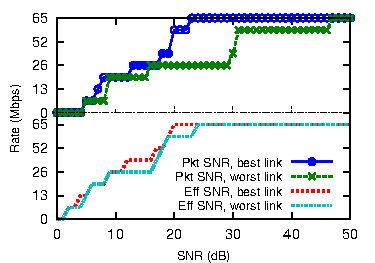
\includegraphics[width=0.95\columnwidth, clip]{figures/embed_ratestep_snr_1x1_90.pdf}%
		\label{fig:snr_rate_step_1x1}%
	}\hspace{0.14\columnwidth}%
	\subfigure[Single spatial stream, three receive antennas (1x3)]{
		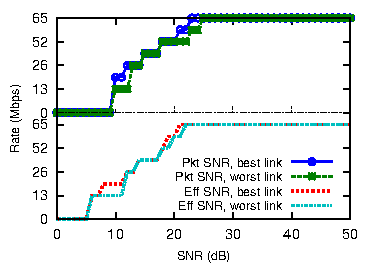
\includegraphics[width=0.95\columnwidth, clip]{figures/embed_ratestep_snr_1x3_90.pdf}%
		\label{fig:snr_rate_step_1x3}%
	}
	
	\vspace{-8pt}
	\subfigure[Two spatial streams, three receive antennas (2x3)]{
		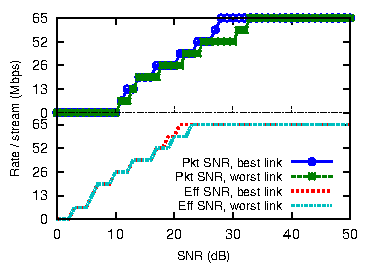
\includegraphics[width=0.95\columnwidth, clip]{figures/embed_ratestep_snr_2x3_90.pdf}%
		\label{fig:snr_rate_step_2x3}%
	}\hspace{0.14\columnwidth}%
	\subfigure[Three spatial streams, three receive antennas (3x3)]{
		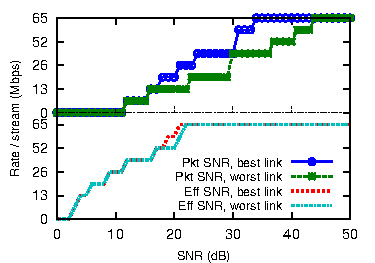
\includegraphics[width=0.95\columnwidth, clip]{figures/embed_ratestep_snr_3x3_90.pdf}%
		\label{fig:snr_rate_step_3x3}%
	}
	\caption{\label{fig:snr_rate_steps}The variation of best rate with SNR over links and antenna configurations. Excepting extremely low and high SNRs, one RSSI-based packet SNR value maps to multiple best rates for different links, %. For the same data, 
while Effective SNR provides a clear indicator of the best rate for nearly all links.}
\vspace{-3pt}
\end{figure*}

\heading{Measurement setup.}
We first measure packet delivery for different antenna configurations over a 20\MHz channel on two \term{iwl5300} testbeds, one at UW CSE and one at Intel Labs Seattle. The 1x1 or SISO configuration corresponds to 802.11a, where each node has a single transmit or receive antenna. In addition we measure configurations with three receive antennas and 1, 2, or 3 spatial streams. These 1x3, 2x3 and 3x3 MIMO configurations are only available with 802.11n. They exploit \emph{spatial diversity} and \emph{spatial multiplexing} to greatly increase performance.

In each test, we send 1500 byte packets as constant bit-rate UDP traffic generated by \term{iperf} at 2\Mbps for 5 seconds. 
We turn off link layer retransmissions to observe the underlying packet delivery rate, and fix the link data rate and the transmit power in each run. Then we collect packet reception rate (PRR) statistics for all 8 rates using 1, 2, and 3 spatial streams as we vary the power between $-$10\dBm and $+$16\dBm in steps of 2\dB.

The receiver also records the CSI and per antenna RSSIs to measure the RF channel for each correctly received packet. Note that CSI is measured during the preamble, so it does not depend on the transmit rate. Similarly, 3x3 CSI gives us the channel between each pair of transmit and receive antennas, so it also implicitly contains 1x1 CSI\@. To get a single SNR value with multiple receive antennas, we first convert the per-antenna RSSIs to SNRs and then sum the SNRs.
This is a straightforward choice for a single spatial stream as it corresponds to receiver processing using MRC~\cite{Goldsmith}.
It is also reasonable for 2- and 3-stream MIMO because the streams are interleaved.

The above testing gives us ground truth data to probe variation across 200 links, 26\dB of transmit power, four antenna configurations ranging from 1x1 to 3x3, and 8 per stream rates (for 24 rates with up to three streams). This covers all of the key variables in our delivery model.

\heading{Result: Rate Confusion.} To understand whether the Effective SNR model accurately predicts packet delivery, we analyze our measurements for the highest supported rate (PRR$\geq$ 90\%) for each link and all NIC settings. The results are shown in \figref{fig:snr_rate_steps}, broken down by antenna configuration. \figref{fig:snr_rate_step_1x1} shows 1x1 rates for both testbeds combined. \figref{fig:snr_rate_step_1x3}--\ref{fig:snr_rate_step_3x3}  show rates for 1x3, 2x3 and 3x3 configurations for the Intel testbed; it is denser than UW and supports MIMO experiments over our NIC's transmit power range.
For each RSSI-based SNR or Effective SNR value, we find the best link (with the fastest best rate) and the worst link (with the slowest best rate). We plot the spread of their fastest rates in these graphs.\footnote{\figref{fig:snr_rate_step_1x3} does not include data for 1x3 at 6.5\Mbps, because very few links experience loss at that rate.}

Ideally, the best and worst lines would overlap completely. %and form a single staircase. 
That is, the highest rate for a given SNR would be the same for the best and worst links. This rate would then be an accurate prediction for the Effective SNR or packet SNR level. Conversely, gaps between the best and worst lines expose confusion about which rate will be the highest rate for that SNR\@.

In the top two lines of the 1x1 and 3x3 cases, we see that the RSSI-based SNR does have a large spread between the best and worst lines. Except for extremely low and high SNRs, nearly all SNRs have at least two and up to five different rates as suitable choices for the best rate. That is, RSSI often poorly indicates rate.

In sharp contrast, %looking at bottom lines in the graphs, 
the two Effective SNR lines overlap almost all the time, and mostly appear to be a single line. This is almost an ideal result. Effective SNR is a clear indicator of best rate. When there is slight separation, the spread is only between rates that use the same modulation but different amounts of coding. These combinations are also close together in our wired experiments. 

Interestingly, we see that RSSI-based predictions are much better for the 1x3 and 2x3 cases, though still not as accurate as Effective SNR, particularly for the high rates. The reason is \emph{spatial diversity}: spare receive antennas gather the received signal and combine to make the channel more frequency-flat. The effect is well-known, though typically not observable using real 802.11 NICs. It suggests that RSSI is a reasonable predictor for an 802.11 configuration with significant diversity. However, observe that RSSI does not transfer well across the antenna modes (as diversity gains and inter-stream interference change unpredictably) which makes this less useful. This is one reason that SISO rate adaptation schemes do not translate to MIMO\@.

We conclude that Effective SNR consistently and accurately indicates the best rate for nearly all links and all configurations without any per-link calibration. From now on, we use the thresholds in these graphs to predict the working rate for any link. They agree with the measured SNRs on a wired link (\figref{fig:snr_prr_attenuator}), which strongly suggests that the Effective SNR captures the fundamental error characteristics of the link. 

Finally, we note that neither Effective SNR nor RSSI performs well at the lowest modulation at low SNRs. We believe this artifact arises from errors in the AGC values reported by the NIC, observed by Judd et al.~\cite{judd_rate_adapt} and confirmed by our data for Intel's hardware.

\heading{Further results.} This results are a subset of those presented in~\cite{halperin_esnr}. Though we do not reproduce them all here, the full paper shows that links viewed through the Effective SNR lens have a narrow transition region, much closer to the wired link model of \figref{fig:snr_prr_attenuator} than the wireless links and packet SNR as in \figref{fig:rssi_predictions}. We also demonstrate that the Effective SNR model enables a sender to accurately prune excess transmit power from a strong link while maintaining high packet delivery.

\subsection{Rate Selection Evaluation}
Having demonstrated that Effective SNR can accurately predict packet delivery for wireless links, we finish our evaluation by exploring its effectiveness as a rate selection algorithm in both single-antenna 802.11a/g and MIMO 802.11n channels. Our goal is to perform as well as the best, already near-optimal 802.11a/g schemes on their home ground, with a method that has the advantages of simplicity, deployability, and generality. Next, we show that our method extends well to 802.11n (MIMO) and so provides ongoing value. At the time we published this work, rate adaptation for 802.11n was an open problem with no published practical schemes, and complex, poorly performing algorithms in Intel's \term{iwlwifi} Linux driver. In future work, we would like to additionally compare to the 802.11n-enabled version of Minstrel released during in late 2010.

\heading{Methodology.} We used trace-driven simulations to compare rate selection or rate adaptation algorithms. A mobile client at UW CSE that is moved at normal walking speed sends short, back-to-back packets to stationary testbed nodes that record the CSI\@. Note that CSI is estimated during the preamble of the packet transmission, independent of the modulation and coding of the payload or the payload length. Therefore, the mobile transmitter can quickly cycle through all antenna configurations (1x3, 2x3 and 3x3) by sending a single short UDP packet at the lowest rate for each configuration. This enables fine grained sampling of the channel every 650\us. The following results are derived from a trace with approximately 85,000 channel measurements taken over 55 seconds, spanning varying RF channels that range from the best 3-stream rates to SISO speeds.

\heading{Algorithms.} We experiment with ESNR, an algorithm based on our model, plus a SampleRate~\cite{Bicket_SampleRate} (with modifications to behave like Minstrel~\cite{minstrel}) and SoftRate~\cite{Vutukuru_SoftRate}, a research algorithm with the best published results. We take advantage of our trace-driven simulations to consider an optimal algorithm, OPT, that has an oracle that knows the true highest rate that can be successfully delivered at any given time. We also consider a Previous-OPT scheme that knows the optimal rate for the previous transmission and uses it for the next packet; it just does not know the future. Since SoftRate and ESNR use an estimate of this previous channel state, and SampleRate infers the recent channel state, they are unlikely to beat Previous-OPT\@. The gap between Previous-OPT and OPT is also likely to be significant because of inherent wireless channel variability.

\heading{Simulator.} We feed this trace to a custom 802.11a/g/n simulator written in a combination of MATLAB and the MIT C++ GNU Radio code. The simulator implements packet reception as shown in \figref{fig:ofdm_decoding}, including demodulation for BPSK through QAM-64, deinterleaving, and convolutional decoding with soft inputs and soft outputs. The measured CSI is interpolated to 56 carriers and serves as the ground truth for the channel, and packets are correctly received when there are no bit errors, or are lost. SampleRate, SoftRate, and ESNR are implemented as described previously. To ensure that ESNR is not given the unrealistic advantage of ground truth CSI, we corrupt the CSI at the level of ADC quantization, which typically induces an error of $\pm$1.5\dB in the output Effective SNRs. SoftRate estimates the BER directly during decoding.

\begin{figure}[t]
      \centering
      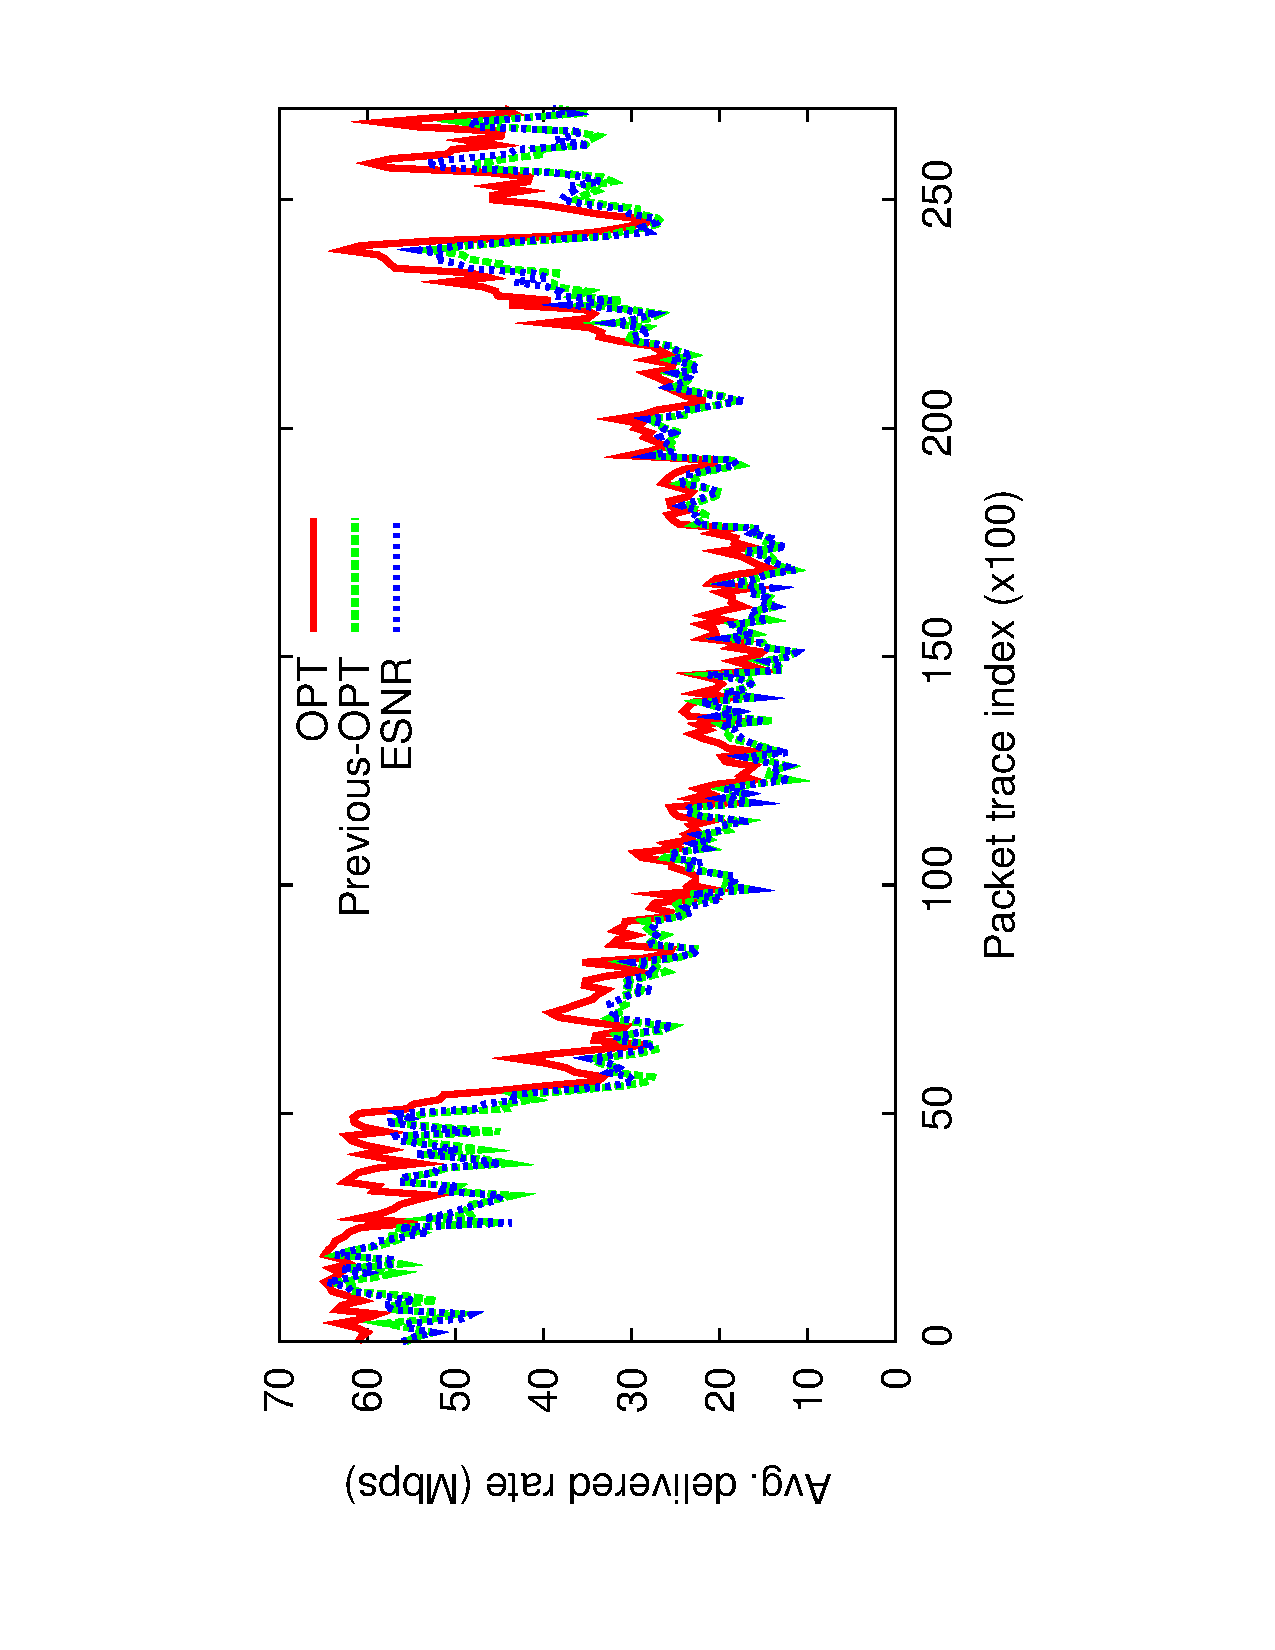
\includegraphics[angle=-90,viewport=120 68 491 760,clip,width=0.95\columnwidth]{figures/siso_rate_time_opt_eff.pdf}
      \caption{\label{fig:siso_rate_time_opt_eff} OPT and ESNR SISO performance in human-speed mobility.}
\end{figure}

\begin{figure}[t]
      \centering
      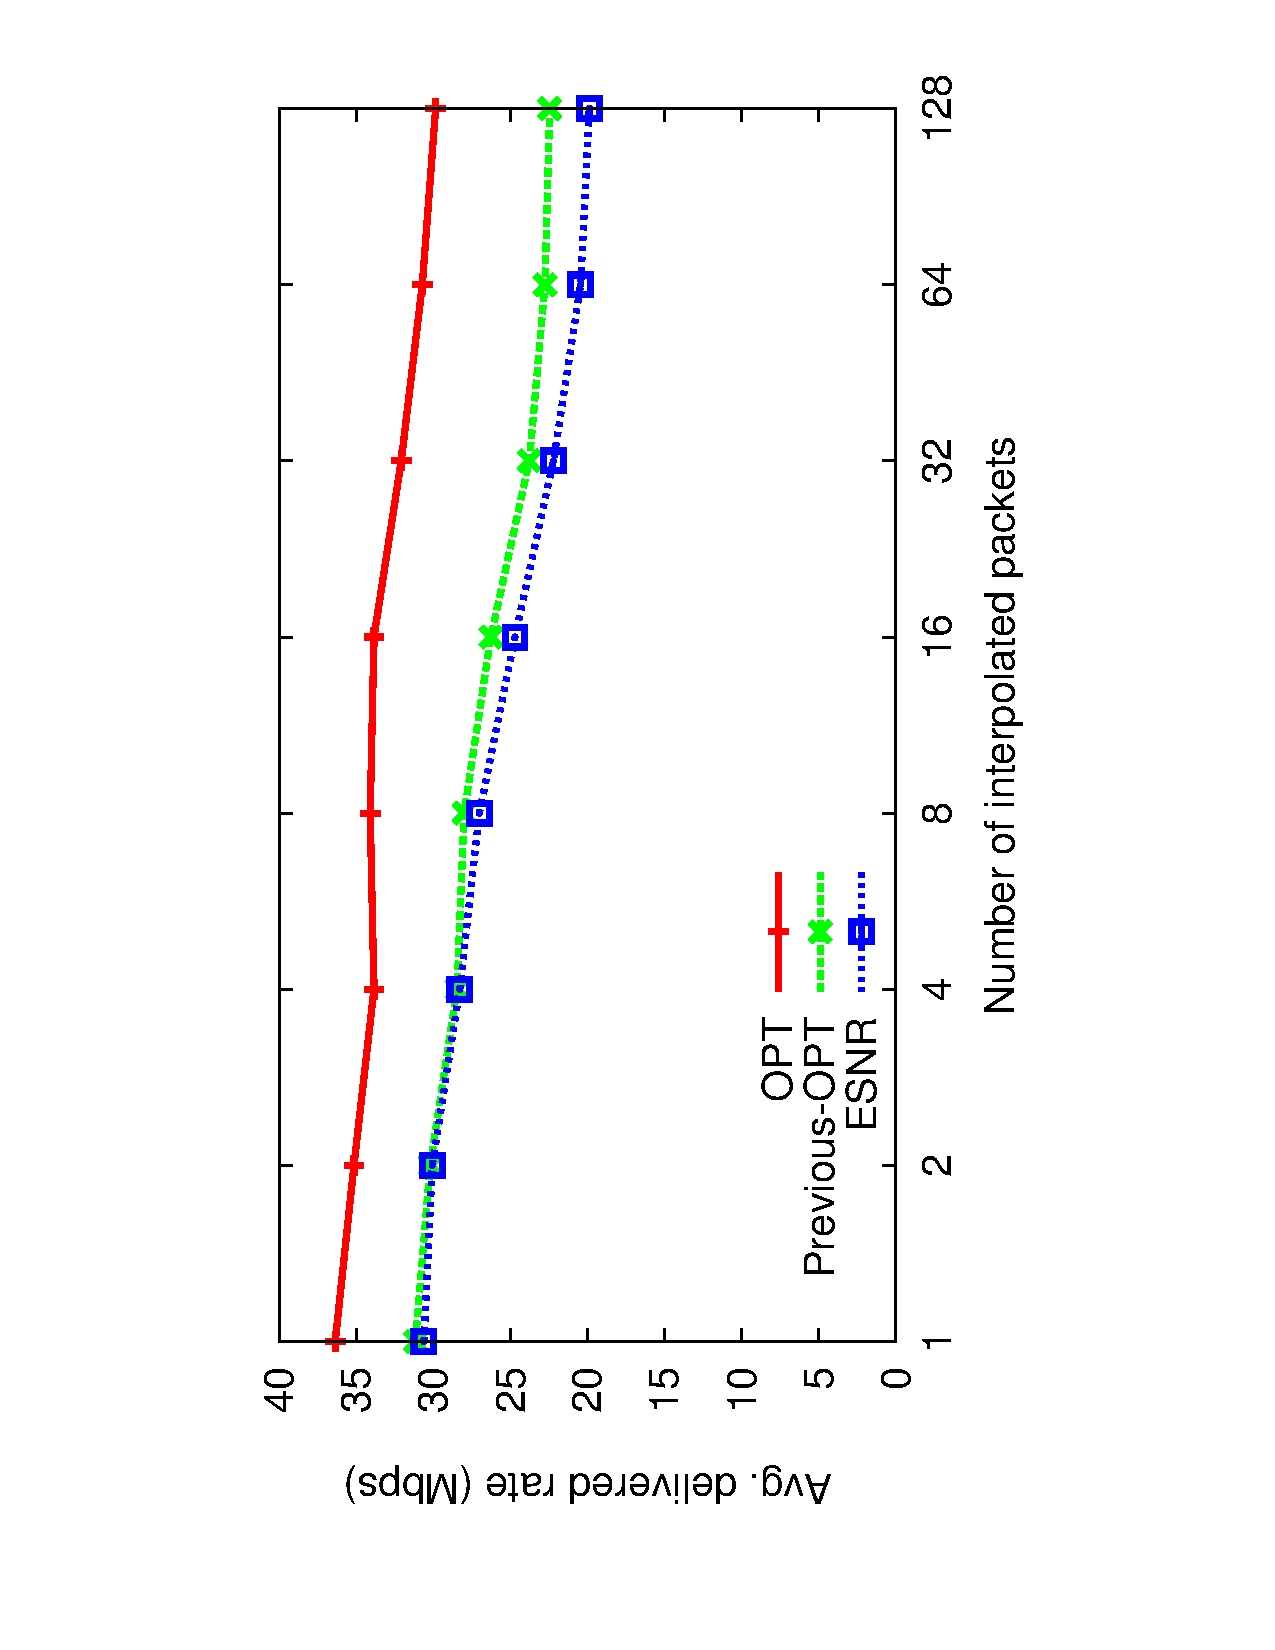
\includegraphics[angle=-90,viewport=120 68 491 760,clip,width=0.95\columnwidth]{figures/siso_rate_skip_opt_eff.pdf}
      \caption{\label{fig:siso_rate_skip_opt_eff} OPT and ESNR SISO performance in fast mobile channels.}
\end{figure}


To vary mobility, we replay the trace at different speeds. For example, 4$\times$ mobility gives ESNR the CSI from every fourth trace record. However, packet reception still uses all trace records. For a packet to be correctly received in the accelerated trace, it must be received over the intermediate records. We require correct reception at $\geq$80\% of the records to allow for coding. This models a varying channel that we can only sample for CSI periodically, as happens when CSI is measured during the packet preamble. SoftRate operates using the 80$^\text{th}$ percentile soft estimate from the range.

We aim to evaluate the ability of these algorithms to respond to changing channel conditions. Thus, our primary metric is the delivered PHY layer rate per trace index. Higher-layer factors such as MAC backoff, link-layer packet aggregation, and TCP reactions to loss, will affect how this rate translates to throughput.

\begin{figure}[p]
      \centering
      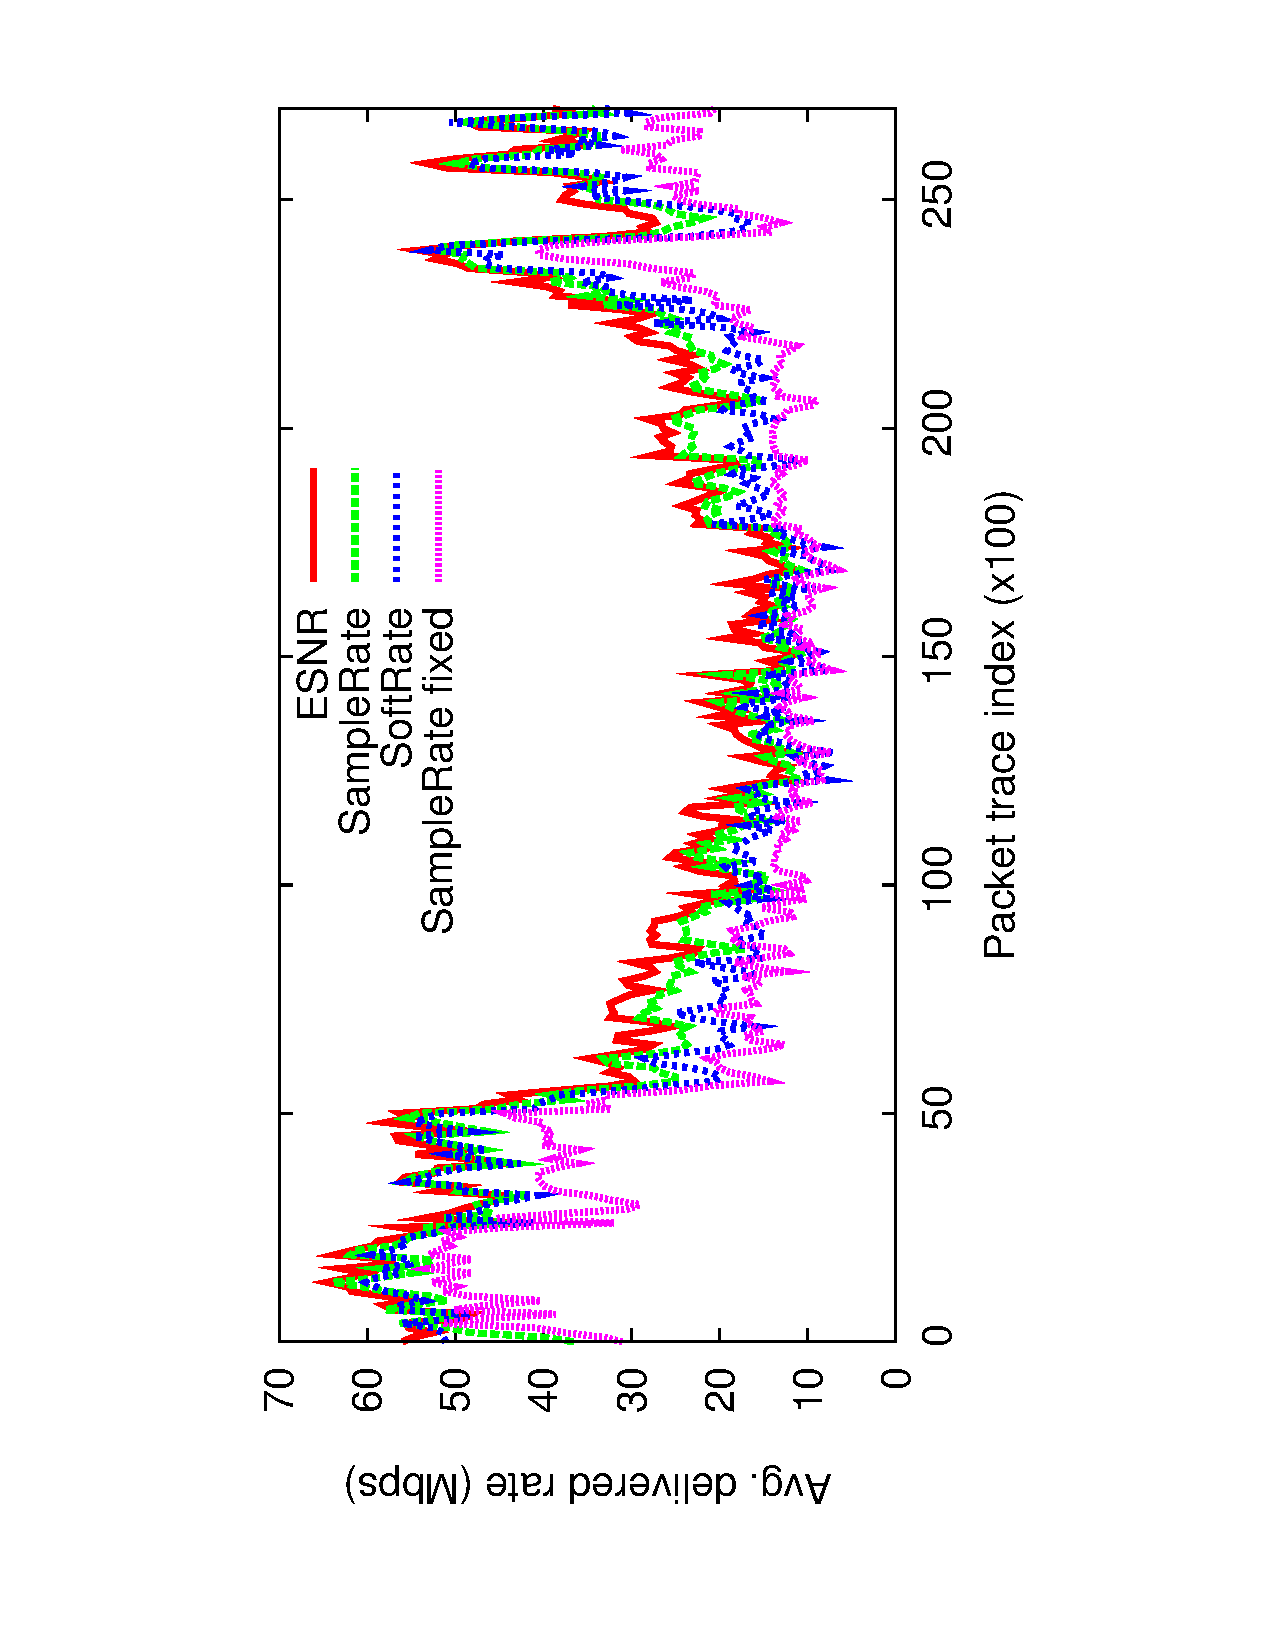
\includegraphics[angle=-90,viewport=120 68 491 760,clip,width=0.95\columnwidth]{figures/siso_rate_time_opt_eff_sr_so.pdf}
      \vspace{-2pt}
      \caption{\label{fig:siso_rate_time_opt_eff_sr_so} ESNR, SampleRate, and SoftRate SISO performance in human-speed mobility.}
      \vspace{-2pt}
\end{figure}

\begin{figure}[p]
      \centering
      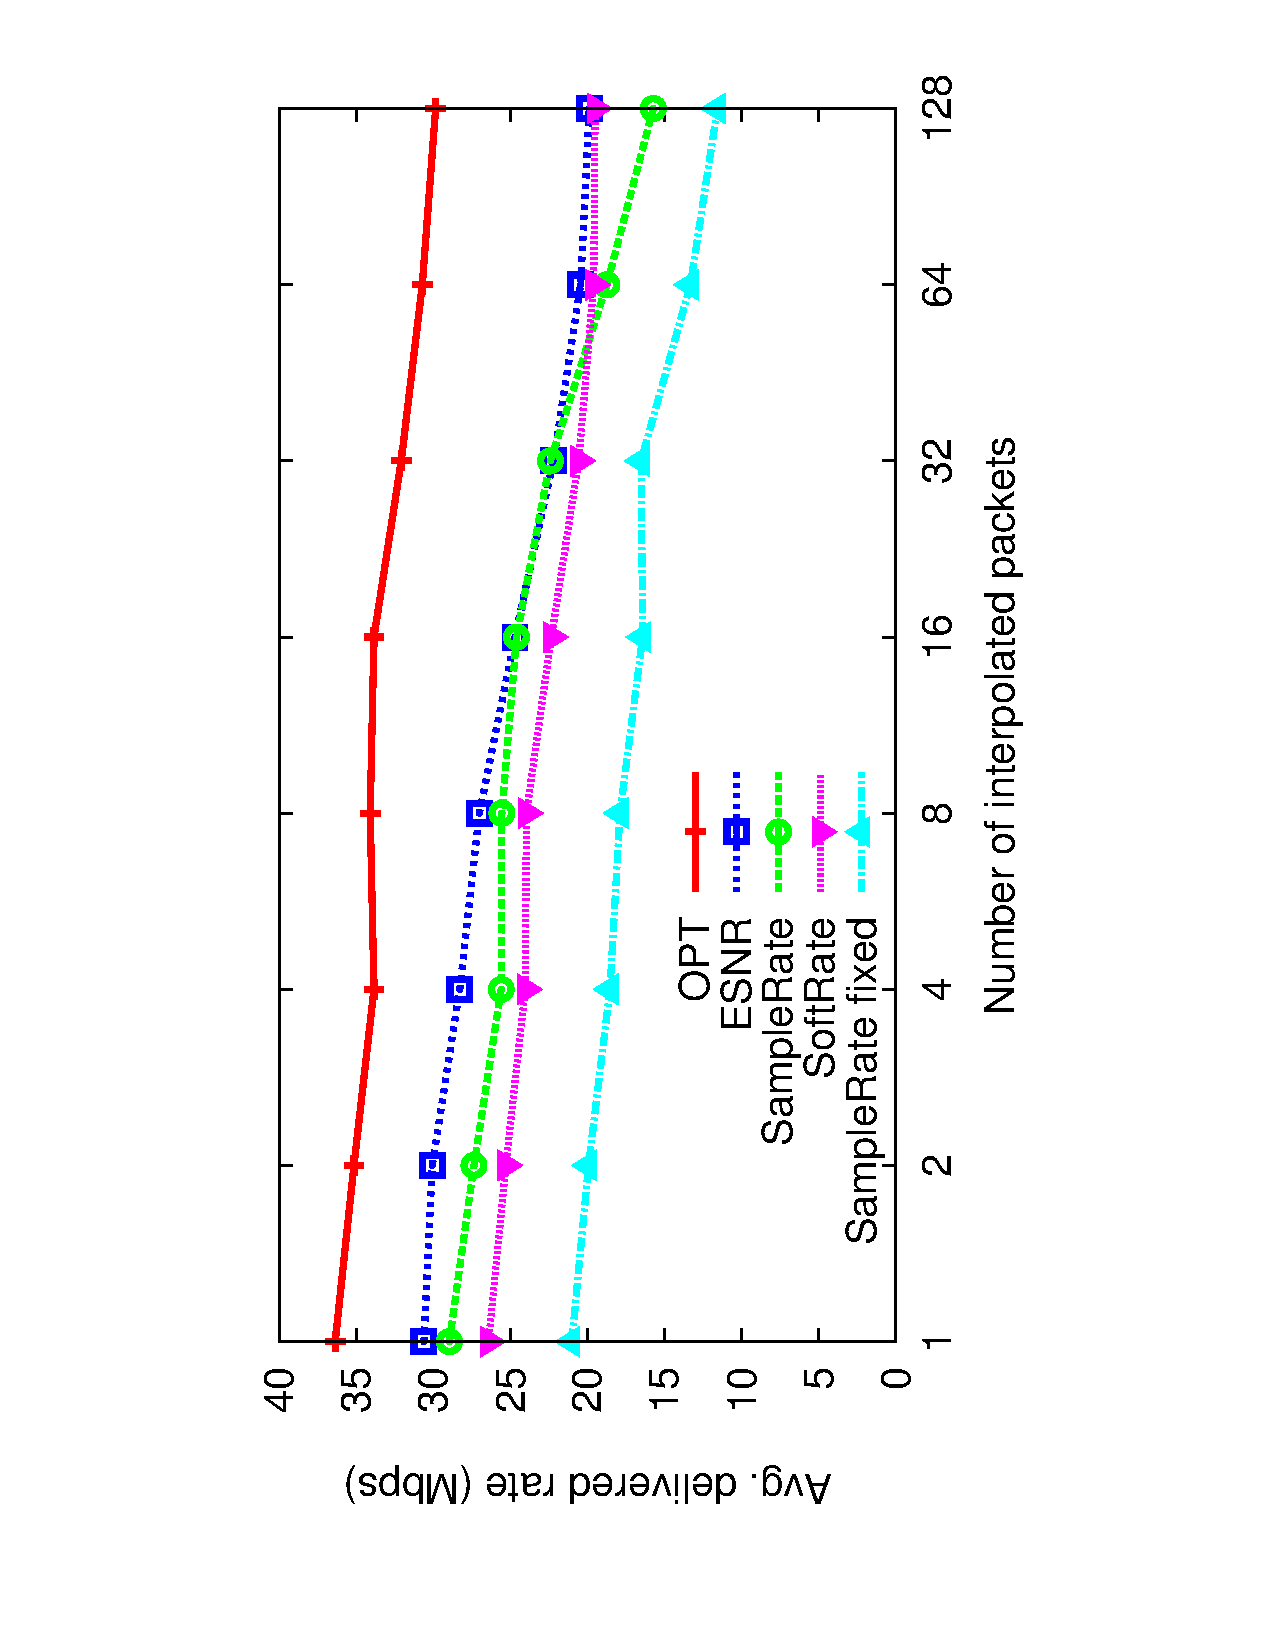
\includegraphics[angle=-90,viewport=120 68 491 760,clip,width=0.95\columnwidth]{figures/siso_rate_skip_opt_eff_sr_so.pdf}
      \vspace{-2pt}
      \caption{\label{fig:siso_rate_skip_opt_eff_sr_so} OPT, ESNR, SampleRate, and SoftRate SISO performance in fast mobile channels.}
      \vspace{-2pt}
\end{figure}


\begin{figure}[p]
      \centering
      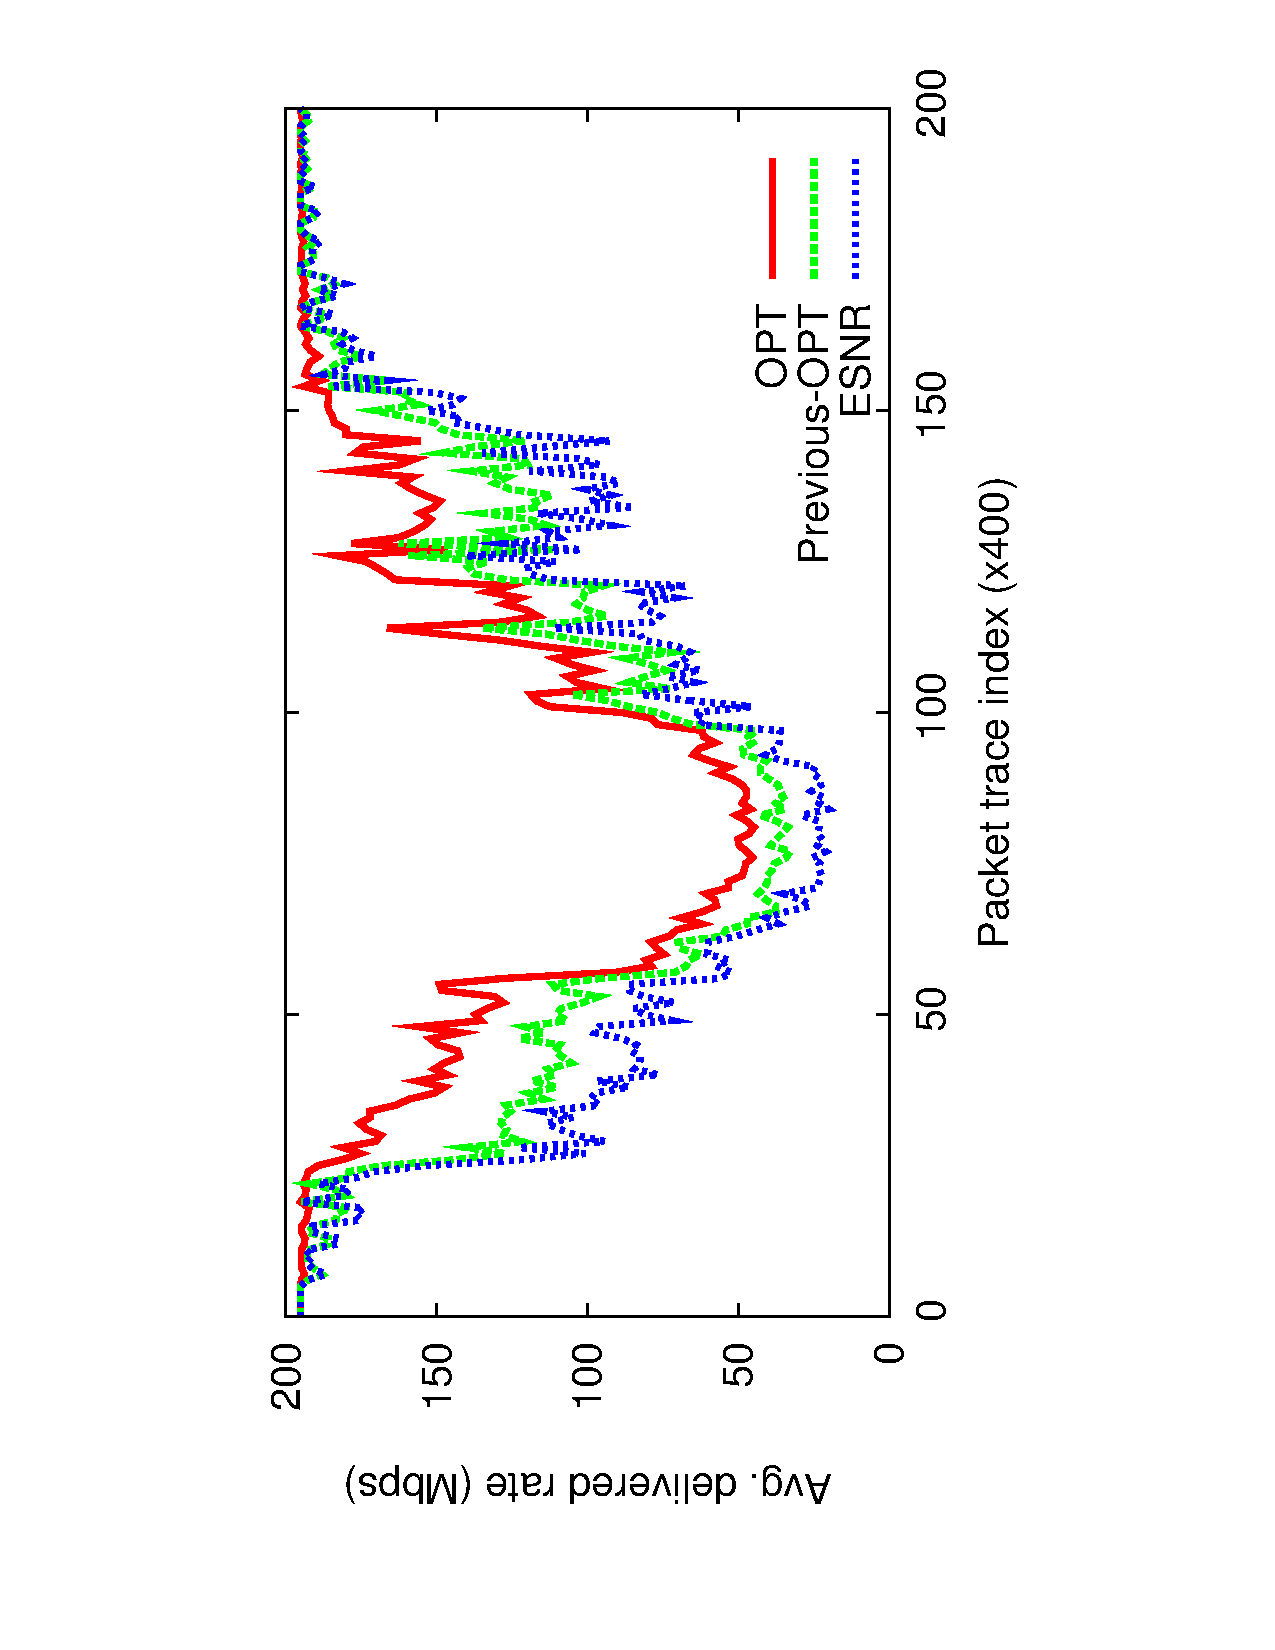
\includegraphics[angle=-90,viewport=125 68 491 760,clip,width=.95\columnwidth]{figures/mimo_skip_time.pdf}
      \vspace{-2pt}
      \caption{\label{fig:mimo_eff_snr_time} OPT and ESNR MIMO performance in human-speed mobility.}
\end{figure}

\begin{figure}[p]
      \centering
      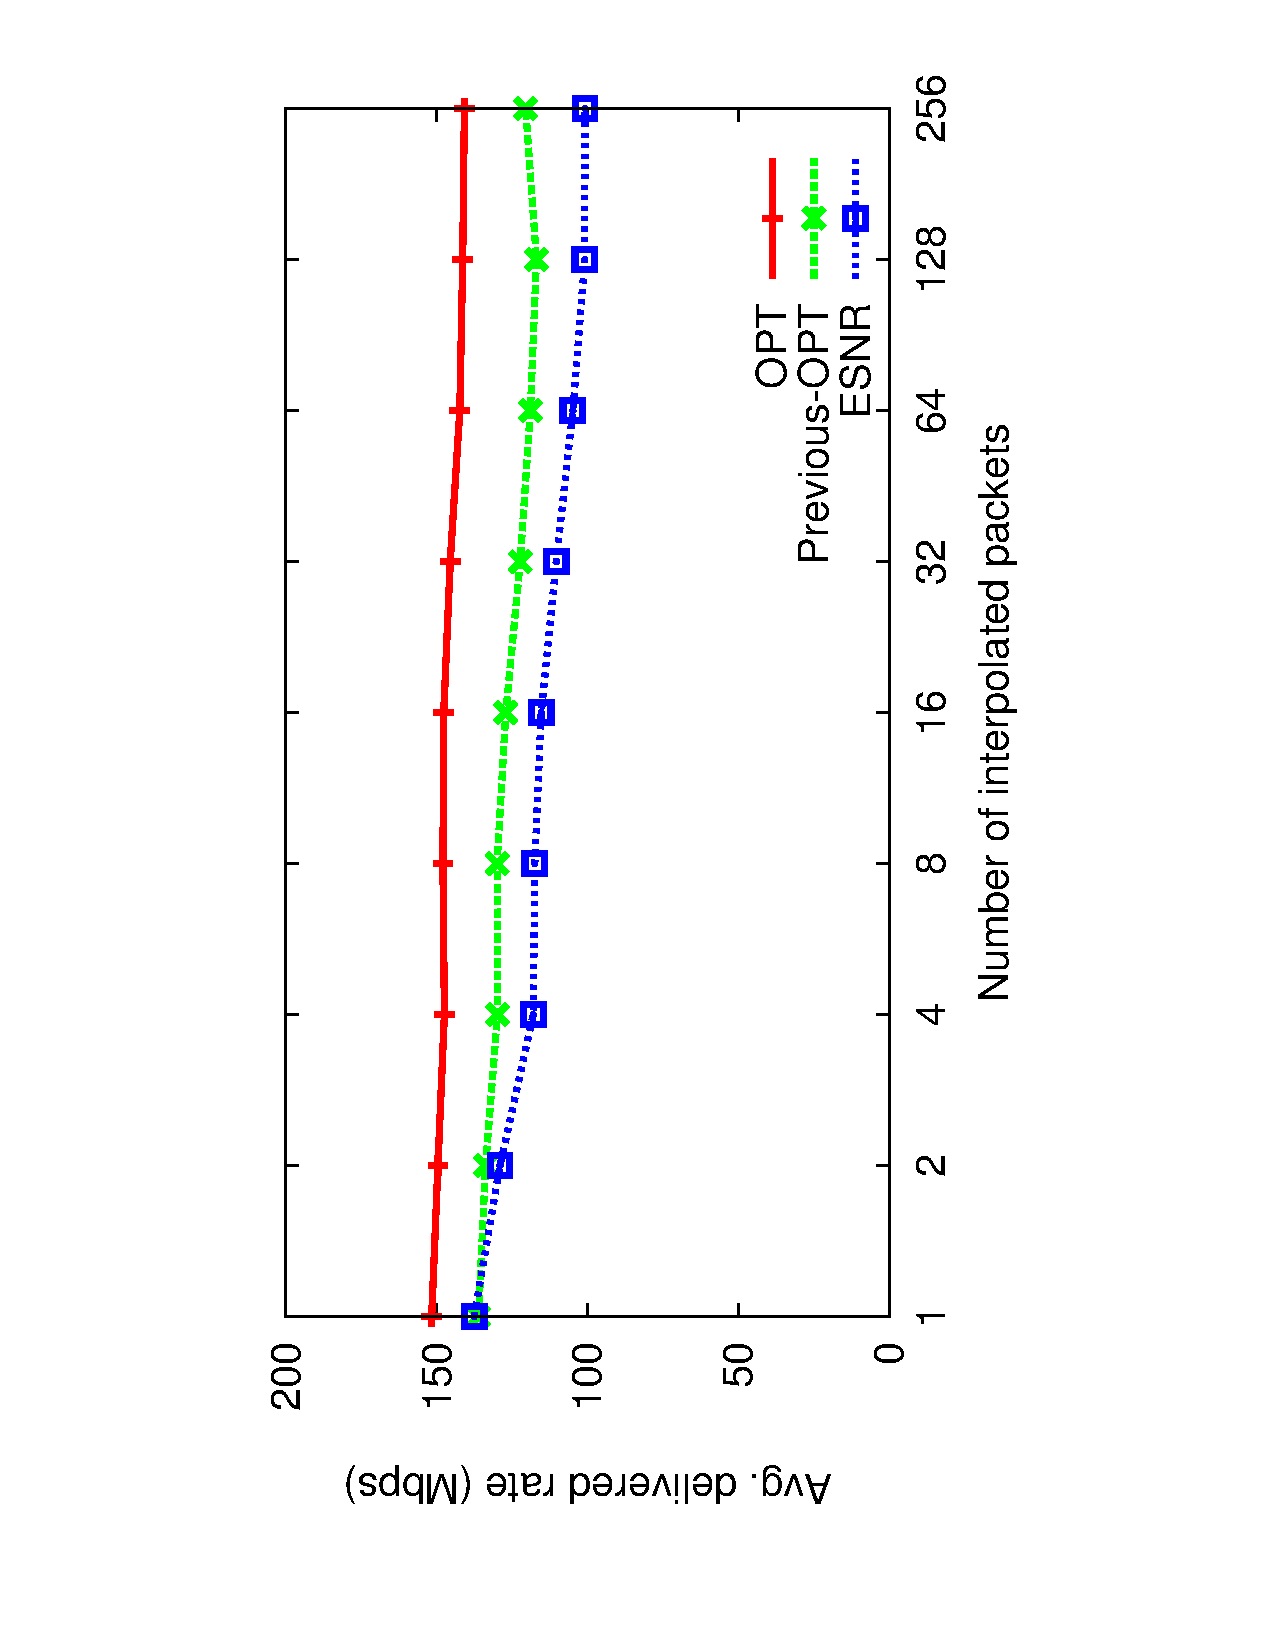
\includegraphics[angle=-90,viewport=125 68 491 760,clip,width=.95\columnwidth]{figures/mimo_rate_skip.pdf}
      \vspace{-2pt}
      \caption{\label{fig:mimo_eff_snr_speedup} OPT and ESNR MIMO performance in faster mobile channels.}
      \vspace{-2pt}
\end{figure}

\heading{SISO Performance.} We first examine the performance of ESNR for SISO rates. \figref{fig:siso_rate_time_opt_eff} shows the rate over time for ESNR and OPT over our trace. The performance metric is the average rate over an interval because each algorithm gets an opportunity to send a packet at the same point in the trace. The rate is averaged over a window of 100 packets to smooth the data for readability. ESNR performs excellently. It is below OPT but consistently overlaps Previous-OPT, which is an upper bound for schemes that track the channel and do not predict the future. ESNR is accurate on 75\% of packets, with the expected 10\% target over-selection.

Next, we compare ESNR with SampleRate and SoftRate %. The corresponding rate versus time and rate versus mobility speedup graphs are shown 
in \figref{fig:siso_rate_time_opt_eff_sr_so} and \figref{fig:siso_rate_skip_opt_eff_sr_so}. While it is hard to separate the lines on the graph, at 1$\times$ speed, ESNR slightly outperforms SampleRate which slightly outperforms SoftRate. These results surprised us: SampleRate performs better than we expected, and SoftRate performs less well.

SampleRate's lagging channel estimate makes it degrade fastest with increasing mobility. However, it maintains a 10--25\% margin with ESNR, still performing well even with large speedups. In deeper analysis, we discovered that dropping rate on retry is an important factor that gives it short-term adaptability. Without this rate fallback (the ``SampleRate fixed'' line), it loses 25--50\% of its performance.

SoftRate has among the slowest falloff with mobility speedup because it directly and accurately measures the channel, and performs the best at maximum speed. However, at slow speeds it is slightly slower on average than SampleRate, though it easily beats a SampleRate without fallback that was the basis for earlier comparisons.\footnote{M. Vutukuru, personal communication, and code inspection.}
We do not believe this gap is fundamental, as SoftRate's post-decoding BER estimate should match or even slightly improve on ESNR\@. Further tuning will likely improve SoftRate. Note that the task for SoftRate is harder in our setting than in the original evaluation. We have added QAM-64 and other coding rates, so it must now chose among 8 SISO rates.

Finally, while the performance differences between schemes are significant, they are always less than a factor of two (ignoring OPT). To put this in perspective, note that other evaluations have reported throughput based on TCP traffic, which will magnify performance gaps by reacting to packet loss.

\heading{MIMO Performance.}
To show the generality of our model, Figures~\ref{fig:mimo_eff_snr_time} and \ref{fig:mimo_eff_snr_speedup} show the performance of an unmodified ESNR algorithm running for 802.11n MIMO rates. These results do not include SampleRate or SoftRate as they are SISO schemes. Instead, we use OPT as our benchmark.
%\figref{fig:mimo_eff_snr_time} and \figref{fig:mimo_eff_snr_speedup} show the rate versus time and rate versus speedup graphs. 
These figures are in the same form as for SISO, except the range of rates has grown by a factor of 3 to support up to 195\Mbps. 

The trends in these graphs are similar to those in the SISO graphs: at human mobility speeds, ESNR tracks Previous-OPT and delivers excellent performance, with 80\% accuracy and 10\% over-selection. In faster mobile channels, there is a slightly larger gap with Previous-OPT for MIMO than for SISO, likely because ESNR must now choose between 24 rates instead of 8. It is more likely to choose rates under the highest rate that would have worked. 

Finally, note that with 3 antennas there are only four two- and three-stream rates over 117\Mbps (130, 156, 175.5 and 195 Mbps). The visible gap between indices 25--50 in \figref{fig:mimo_eff_snr_time} reflects only the difference between 1 or 2 rates of potentially different antenna modes. Taken together, these results imply that ESNR's MIMO performance is highly competitive.

\heading{Antenna Selection.}
One strength of our model is that it can accommodate choices other than rates. This lets us add other functionality to ESNR without increasing complexity. One enhancement is to select the best transmit antenna when there are spare antennas.
An 802.11n AP can select antennas to use to send packets to a legacy 802.11a/g client (plus use all antennas to receive packets). With three antennas to choose from, the expected gain in SNR is a little over 2.5\dB~\cite{Goldsmith}. This is often enough to advance to a higher rate. We ran a version of SISO ESNR that chose the antenna with the highest ESNR for the next transmission. This gave a gain in the average rate of 5\%.  For comparison, OPT achieved a 10\% increase by always knowing which antenna was best. No other rate adaptation schemes directly support these enhancements.

\heading{Prototype Implementation.} Finally, we implemented a version of ESNR that randomly probes other antenna modes to collect CSI and that also sends Effective SNR estimates back to the transmitter, and ran it online against SampleRate in human-scale mobility. We found that the probing and feedback have little penalty, and our results match the simulator: the two algorithms are separated by a small (5--10\%) margin.

\subsection{Summary} In our preliminary work, we built an experimental platform for 802.11n measurements using commodity Intel Wi-Fi NICs. A key feature of this tool is its ability to measure fine-grained RF channel state at the level of subcarriers and antenna pairs. We used the collected CSI to implement an 802.11n Effective SNR model and demonstrated that it can effectively predict packet delivery. In preliminary work, we explored rate and MIMO mode selection, antenna selection, and transmit power control for a single wireless link. We believe that the same tools can likely be applied to many other problems for a single link and also to help multiple links coexist. As part of our proposed work in the following section, we plan to use Effective SNR as a tool in our network architecture for the techniques we've already demonstrated, and also to explore its use for other relevant search problems.